%----------------------------------------------------------------------------------------
%	PACKAGES AND THEMES
%----------------------------------------------------------------------------------------
\documentclass[aspectratio=169,xcolor=dvipsnames]{beamer}
\usetheme{Simple}
\usepackage{hyperref}
\usepackage{hyperref}
\usepackage{graphicx} % Allows including images
\usepackage{booktabs} % Allows the use of \toprule, \midrule and \bottomrule in tables
\usepackage{graphicx}
%----------------------------------------------------------------------------------------
%	TITLE PAGE
%----------------------------------------------------------------------------------------

% The title
\title[short title]{Project Update Presentation}
\subtitle{Semi-supervised Sequence Learning}

\author[Sanjay K V] {Sabiha Sultana\inst{1}, Piyakorn Munegan\inst{2},\\ Sanjay Kanakkot Viswanathan\inst{3},\break Mohammed Rizwan Amanullah\inst{4}}
\institute[NTU] % Your institution may be shorthand to save space
{
    % Your institution for the title page
    Department of Computing, \\
    Macquarie University 
    \vskip 3pt
}
\date{\today} % Date, can be changed to a custom date


%----------------------------------------------------------------------------------------
%	PRESENTATION SLIDES
%----------------------------------------------------------------------------------------

\begin{document}

\begin{frame}
    % Print the title page as the first slide
    \titlepage
\end{frame}

\begin{frame}{Overview}
    % Throughout your presentation, if you choose to use \section{} and \subsection{} commands, these will automatically be printed on this slide as an overview of your presentation
    \tableofcontents
%------------------------------------------------
%Overview
%------------------------------------------------
\begin{itemize}
        \item In this paper, we are replicating project which aims on unlabelled data to improve sequence learning with Recurrent network \break
        \textbf{Previous approach}
        - \textbfUsing Bag of words on IMDB Datasets \break
    \end{itemize}

 %Adding picture
  \begin{figure} 
  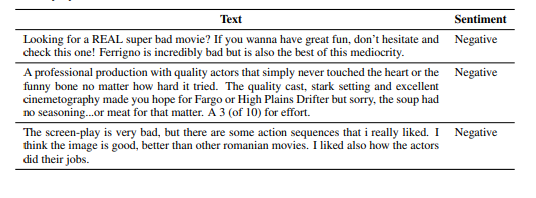
\includegraphics[width=250]{Introduction.png}
\end{figure}
%------------------------------------------------
\textbf{Current approach}\break
        - (LM-LSTM) Language modelling. Predict what comes next in sequence.\break
        - (SA-LSTM) Sequence auto encoder. Reads input sequence into vectors and \break predict the input sequence again.
 
  
\end{frame}
%------------------------------------------------
%Replication1
%------------------------------------------------

\begin{frame}{Sentiment analysis experiments with IMDB}
    \begin{itemize}
        \item Requirements: AWS(EC2) with Python 3, tensorflow v 1.15.5
        \item Dataset: IMDB movie review dataset\break 
            - Training set: 25,000 labeled and 50,000 unlabeled reviews.\break 
            - Test set: 25,000 labeled reviews.\break
            - The average length of each document is 241 words. 
        \newline
        \newline
         \begin{figure2}
            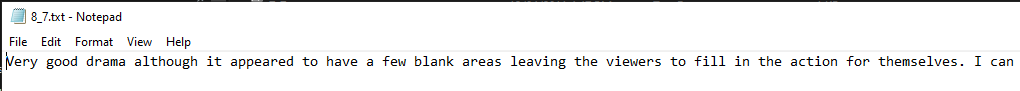
\includegraphics[width=400]{positive labblled review.PNG}
        \end{figure2}
    \end{itemize}
\end{frame}

%------------------------------------------------




%------------------------------------------------
%Replication2
%------------------------------------------------

\begin{frame}{Sentiment analysis experiments with IMDB cont.}
    \begin{itemize}
         \begin{figure2}
            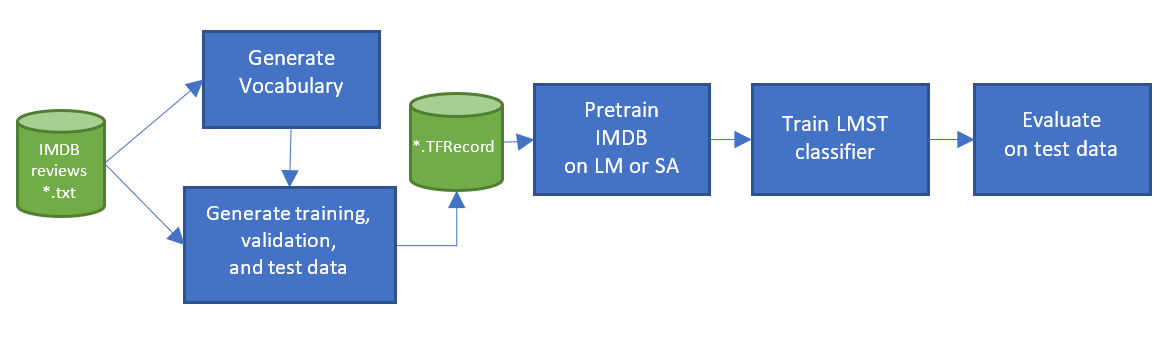
\includegraphics[width=400]{replicationFlow2.PNG}
        \end{figure2}
        \newline
        \newline
        - Accuracy of model LM-LSTM on 10\% of the size of the original dataset is  0.52 \break
    \end{itemize}
\end{frame}

%------------------------------------------------


%------------------------------------------------
% Sanjay Issues Explanation in details
%------------------------------------------------
\begin{frame}{Output - Representation}
    % Throughout your presentation, if you choose to use \section{} and \subsection{} commands, these will automatically be printed on this slide as an overview of your presentation
    \tableofcontents
%------------------------------------------------
%Overview
%------------------------------------------------

 %Adding picture
 
  \begin{figure}
   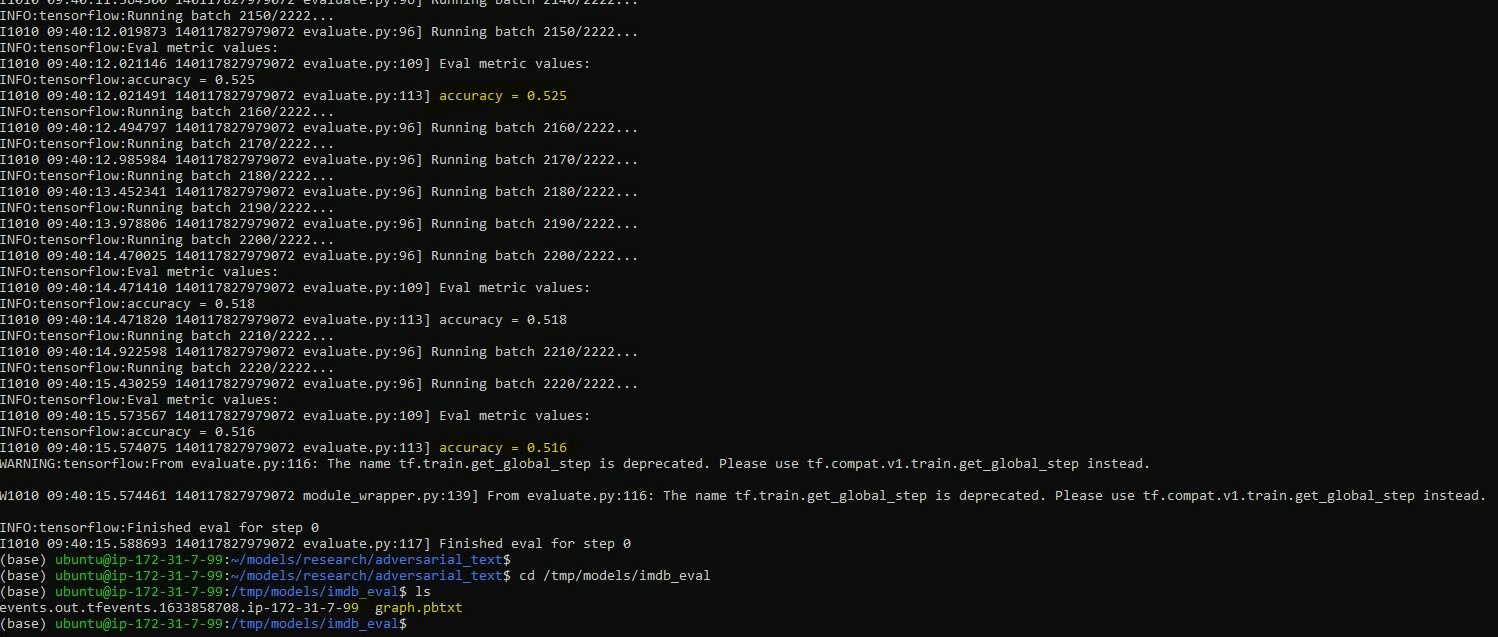
\includegraphics[width=430]{Accuracy_evaluation.jpg}
      \caption{Accuracy got after running Evaluate.py file}
\end{figure}


\end{frame}
%------------------------------------------------




%------------------------------------------------
% Sanjay Issues - Slide 1
%------------------------------------------------

\begin{frame}{Issue Analysis and Solutions}
    \begin{columns}[c] % The "c" option specifies centered vertical alignment while the "t" option is used for top vertical alignment

        \column{.60\textwidth} % Left column and width
        \textbf{The Issues Faced}
        \begin{enumerate}
            \item Process Requirement for LSTM-RNN is huge.
            \item Not Getting the Accuracy as expected.
            \item AWS kills the process due to memory issues.
            \item Eg : Took ~2 days to process with half Data.
            \item Installing dependencies\\ Eg: \alert{Tensor Flow 1.15.5, Wget,nltk,pinkt} 
            \item Filtering/ down sizing the file.
        \end{enumerate}

        \column{.5\textwidth} % Right column and width
         As a workaround during replication of\\ the project
         we reduced the model size\\ to 10 Percentage and 
         set parameters to low \\and ran the process
         which resulted in\\ getting \alert{accuracy of 0.52} with nearly \\ \textbf{7 hours of time.}\\
         The folders neg, pos, unsup where \\ filtered and \alert{downsized 
         to 10 percentage}\\ of the raw data.


    \end{columns}
\end{frame}
%------------------------------------------------
   



%------------------------------------------------
% Sanjay Issues Explanation in details
%------------------------------------------------
\begin{frame}{Explanation - Issues}
    % Throughout your presentation, if you choose to use \section{} and \subsection{} commands, these will automatically be printed on this slide as an overview of your presentation
    \tableofcontents
%------------------------------------------------
%Overview
%------------------------------------------------

 %Adding picture
  \begin{figure}
   \caption{Error encountered when ran the file without scaling down}
   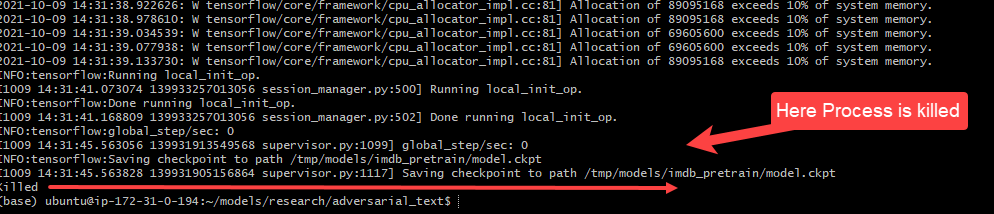
\includegraphics[width=450]{Killed-aws.png}
\end{figure}

\textbf{Scaled-down}
        - We reduced the parameter on the code to proceed further. \break
        - \alert{rnn-cell size, batch-size, max-steps} are the parameters changed.

  
\end{frame}
%------------------------------------------------



%------------------------------------------------
% Sanjay Issues Explanation in details
%------------------------------------------------
\begin{frame}{Explanation - Issues Solution}
    % Throughout your presentation, if you choose to use \section{} and \subsection{} commands, these will automatically be printed on this slide as an overview of your presentation
    \tableofcontents
%------------------------------------------------
%Overview
%------------------------------------------------

 %Adding picture

  \begin{figure}
   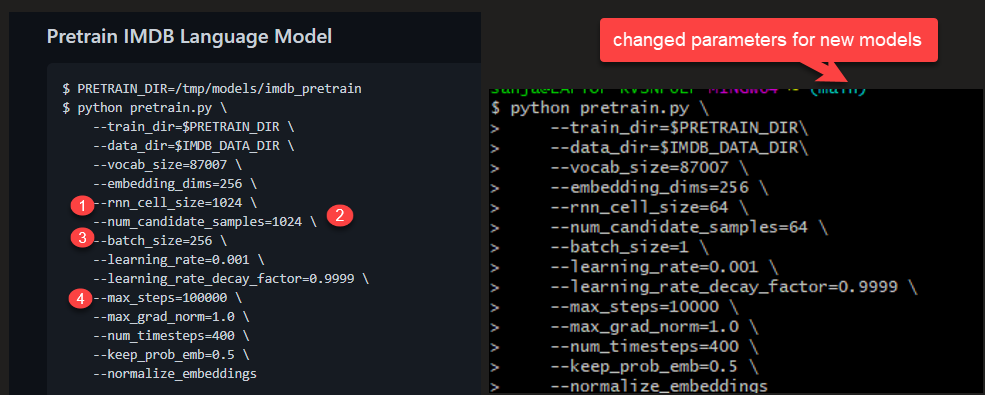
\includegraphics[width=420]{new_model_1.png}
      \caption{On left the Default parameter, On right Parameters we used for replication}
\end{figure}


\end{frame}
%------------------------------------------------

%------------------------------------------------
%justification of original work
%------------------------------------------------

\begin{frame}{New Data Generation}
    \begin{itemize}
        \item As part of data creation, we have scrapped amazon.in website using selenium and Beautiful soup for product listing and product reviews.
        \item We have extracted product listing and product reviews information for ten categories. \break 
            - After extraction, we are manually tagging the product listing and reviews. \break
            - For product listing we are manually tagging the company names and for product review which having positive and negative reviews.\break  
     \item \alert{Issues faced:} For certain product categories, the alignment of the page is changing as a result, we had to find common \textbf{xpath} to find and extract product listing for all the ten categories.
        \newline
        \newline

    \end{itemize}
\end{frame}


%----------------------------------------------------------------------------------------


%------------------------------------------------
%New Data Gen : Pic
%------------------------------------------------

\begin{frame}{New Data Generation: Representation}

         \begin{figure2}
         \caption{Sample Output file after web scrapping}
            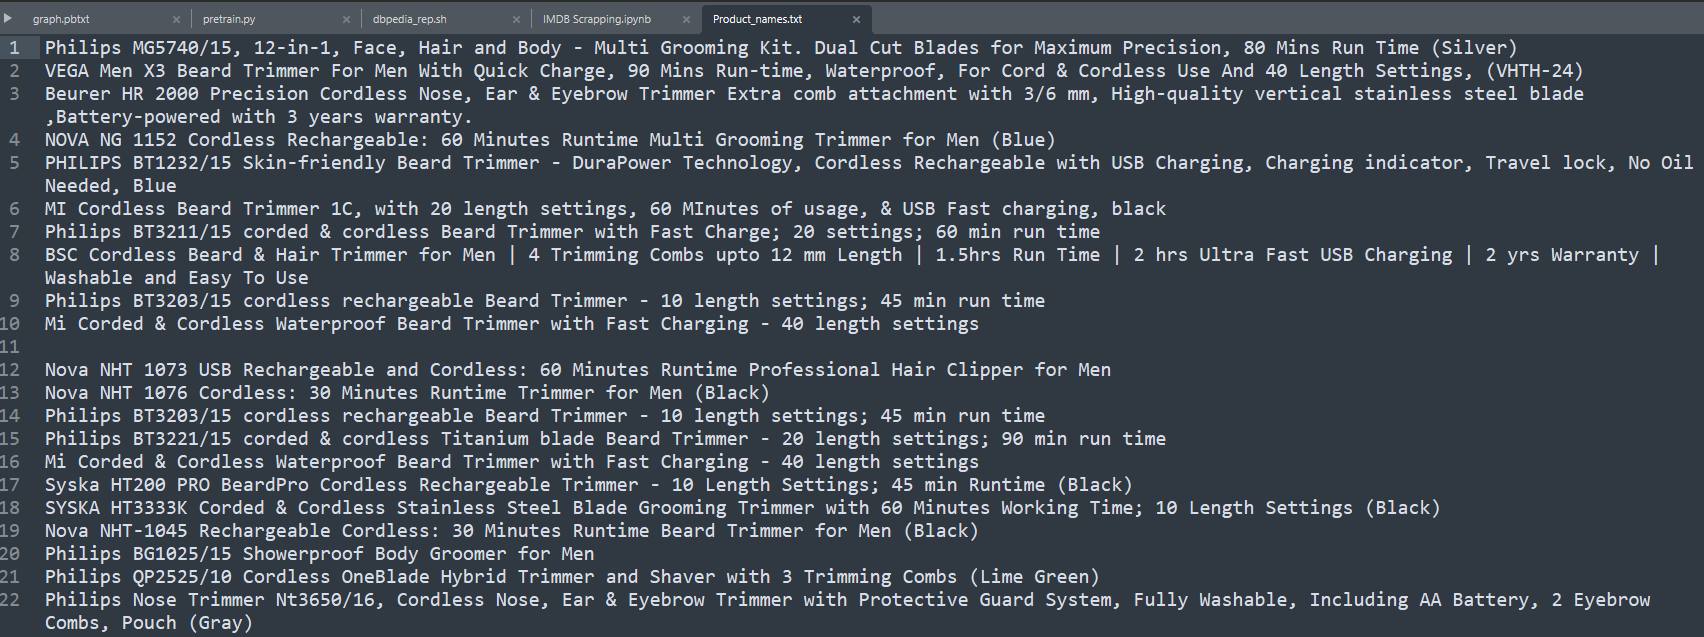
\includegraphics[width=430]{Product_listing.png}
            
        \end{figure2}
\end{frame}


%----------------------------------------------------------------------------------------
\begin{frame}
    \Huge{\centerline{The End}}
\end{frame}

%----------------------------------------------------------------------------------------

\end{document}